\documentclass[a4paper,12pt]{article}

% defining margin for the document
\usepackage[margin=1.00in]{geometry}

\usepackage{algorithm}
\usepackage[utf8]{inputenc}
% \usepackage{arevmath}
\usepackage[noend]{algpseudocode}

% these packages are used for images
\usepackage{graphicx}

\title{SOEN 6011 - Scientific Calculator}
\author{Saraswati Saud \\
Student ID: 40115097}
\date{}
\begin{document}
\maketitle
\section{Problem 1: Gamma function, $\Gamma$ (x)}
    \subsection{Description}
    The gamma function represented by $\Gamma$(x), is an extension of the factorial function to complex numbers. It is defined for all the complex numbers except the non-positive integers.\\ \\
    Specifically, $\Gamma$(n) = (n-1)! where n $\textgreater$ 0.

    \subsection{Domain}
    Any complex number that is not a negative integer is in the domain of the function.\\
    So, the domain of the Gamma function is (0, +$\infty$).
    
    \subsection{Co-domain}
    The co-domain is the set of all real numbers (-$\infty$, +$\infty$).
    
    \subsection{Characteristics of Gamma Function}
    \begin{enumerate}
        \item The gamma function is uniquely defined for all positive integers and complex numbers with positive real parts.
        \item For real values of argument ‘n’, the value of the gamma function $\Gamma$(n) are real (or infinity). The gamma function is not equal to zero.
        \item $\Gamma$(n+1) = n!, for integer n $\textgreater$ 0.
        \item $\Gamma$(n+1) = n $\Gamma$(n) (function equation).
    \end{enumerate}
    
    \begin{thebibliography}{}
        \bibitem{}
        MathWorld: Gamma Function
        \\\texttt{https://mathworld.wolfram.com/GammaFunction.html}
        \bibitem{}
        Geeksforgeeks
        \\\texttt{https://www.geeksforgeeks.org/gamma-function}
    \end{thebibliography}
    
    \newpage
    
\section{Problem 2: Requirements Specification}
    \subsection{Definitions and Abbreviations}
    \begin{center}
    \begin{tabular}{ |p{3cm} | p{10cm}| }
        \hline
        \textbf{Terms} & \textbf{Definitions} \\
        \hline
        FR & Functional Requirement \\
        \hline
        NFR & Non-Functional Requirement \\
        \hline
        User & Someone who interacts with the system \\
        \hline
        System & Software Program for calculation of Gamma Function \\
        \hline
    \end{tabular}
    \end{center}

    \subsection{Constraints and Assumptions}
    \begin{itemize}
        \item User should provide input for ‘x’.
        \item Based on the function characteristics, the value of ‘x’ should either be positive integer or half-integer value.
        \item The input value cannot be 0.
        \item The output will always be a positive decimal.
    \end{itemize}

    \subsection{Requirements}
        \subsubsection{Functional Requirements}
        \begin{tabular}{ |p{4cm} | p{11cm}| }
            \hline
            \textbf{ID:} & FR1\\
            \textbf{TYPE:} & Functional\\
            \textbf{VERSION:} & 1.0\\
            \textbf{DIFFICULTY:} & Easy\\
            \textbf{PRIORITY:} & 1\\
            \textbf{OWNER:} & Saraswati Saud\\
            \textbf{DESCRIPTION:} & System should prompt the user to enter the value of ‘x’. \\
            \textbf{RATIONALE:} & To get user input and start calculation. \\
            \hline
        \end{tabular}
        \\[10pt]
        \begin{tabular}{ |p{4cm} | p{11cm}| }
            \hline
            \textbf{ID:} & FR2\\
            \textbf{TYPE:} & Functional\\
            \textbf{VERSION:} & 1.0\\
            \textbf{DIFFICULTY:} & Medium\\
            \textbf{PRIORITY:} & 2\\
            \textbf{OWNER:} & Saraswati Saud\\
            \textbf{DESCRIPTION:} & System should display an error message when entered value is not   a number. \\
            \textbf{RATIONALE:} & For calculations, input should only be numbers. \\
            \hline
        \end{tabular}
        \\[10pt]
        \begin{tabular}{ |p{4cm} | p{11cm}| }
            \hline
            \textbf{ID:} & FR3\\
            \textbf{TYPE:} & Functional\\
            \textbf{VERSION:} & 1.0\\
            \textbf{DIFFICULTY:} & Difficult\\
            \textbf{PRIORITY:} & 1\\
            \textbf{OWNER:} & Saraswati Saud\\
            \textbf{DESCRIPTION:} & System should display an error message if a user entered negative, zero or positive non-half integer. \\
            \textbf{RATIONALE:} & For calculations, input should only be positive integer or half-integer value. \\
            \hline
        \end{tabular}
        \\[10pt]
        \begin{tabular}{ |p{4cm} | p{11cm}| }
            \hline
            \textbf{ID:} & FR4\\
            \textbf{TYPE:} & Functional\\
            \textbf{VERSION:} & 1.0\\
            \textbf{DIFFICULTY:} & Easy\\
            \textbf{PRIORITY:} & 3\\
            \textbf{OWNER:} & Saraswati Saud\\
            \textbf{DESCRIPTION:} & User should have an option to exit the program anytime during the use. \\
            \textbf{RATIONALE:} & If user is done with the calculations. \\
            \hline
        \end{tabular}

        \subsubsection{Non-Functional Requirements}
        \begin{tabular}{ |p{4cm} | p{11cm}| }
            \hline
            \textbf{ID:} & NFR1\\
            \textbf{TYPE:} & Non-Functional\\
            \textbf{VERSION:} & 1.0\\
            \textbf{DIFFICULTY:} & Medium\\
            \textbf{PRIORITY:} & 2\\
            \textbf{OWNER:} & Saraswati Saud\\
            \textbf{DESCRIPTION:} & The error message displayed should be appropriate and helpful for the user. \\
            \textbf{RATIONALE:} & User should be able to know what went wrong. \\
            \hline
        \end{tabular}
        \\[10pt]
        \begin{tabular}{ |p{4cm} | p{11cm}| }
            \hline
            \textbf{ID:} & NFR2\\
            \textbf{TYPE:} & Non-Functional\\
            \textbf{VERSION:} & 1.0\\
            \textbf{DIFFICULTY:} & Easy\\
            \textbf{PRIORITY:} & 3\\
            \textbf{OWNER:} & Saraswati Saud\\
            \textbf{DESCRIPTION:} & The text-based interface should be user friendly. \\
            \textbf{RATIONALE:} & It should be easy for the user to use the system. \\
            \hline
        \end{tabular}
        \\[10pt]
        \begin{tabular}{ |p{4cm} | p{11cm}| }
            \hline
            \textbf{ID:} & NFR3\\
            \textbf{TYPE:} & Non-Functional\\
            \textbf{VERSION:} & 1.0\\
            \textbf{DIFFICULTY:} & Medium\\
            \textbf{PRIORITY:} & 2\\
            \textbf{OWNER:} & Saraswati Saud\\
            \textbf{DESCRIPTION:} & The displayed result should be as accurate as possible. \\
            \textbf{RATIONALE:} & Incorrect output should not be displayed. \\
            \hline
        \end{tabular}
        \\[10pt]
        \begin{tabular}{ |p{4cm} | p{11cm}| }
            \hline
            \textbf{ID:} & NFR4\\
            \textbf{TYPE:} & Non-Functional\\
            \textbf{VERSION:} & 1.0\\
            \textbf{DIFFICULTY:} & Difficult\\
            \textbf{PRIORITY:} & 1\\
            \textbf{OWNER:} & Saraswati Saud\\
            \textbf{DESCRIPTION:} & Calculation time should be less than 1 second. \\
            \textbf{RATIONALE:} & Waiting a long time for the output might not be desired for the user. \\
            \hline
        \end{tabular}

\newpage
\section{Problem 3: Algorithm and Pseudocode}
    Following are the algorithms and the pseudo-codes of function F4, $\Gamma(x)$:
    \begin{algorithm}
    \caption{Recursive Approach - $\Gamma(x)$ }
    \begin{algorithmic}
    \Procedure{$functionF4$}{$x$}
        \State \textbf{in: } double x
        \State \textbf{out: } double result
        \If{(x $<$ 0)}
            \Return "Wrong Input"
        \Else \If{(x == x.5)}
         \State result = halfFactInteger(x)
            \Else
            \State result = factInteger(x)
            \EndIf
        \State
        \Return result
        \EndIf
    \EndProcedure
    \\
    \Procedure{$halfFactInteger$}{$x$}
    \State \textbf{in: } double x
    \State \textbf{out: } double result
    \If{(($x == 0.5$)}
    \State \Return 1.77
        \Else
    \State \Return $(x-1) * halfFactInteger(x-1)$
    \EndIf
    \EndProcedure
    \\
    \Procedure{$factInteger$}{$x$}
    \State \textbf{in: } double x
    \State \textbf{out: } double result
    \If{(($x == 1$)}
    \State \Return 1
        \Else
    \State \Return $(x-1) * factInteger(x-1)$
    \EndIf
    \EndProcedure
    \\
    \end{algorithmic}
    \end{algorithm}

    \newpage
    % second logic
    \begin{algorithm}
    \caption{Iterative Approach - $\Gamma(x)$ }
    \begin{algorithmic}
    \Procedure{$functionF4$}{$x$}
        \State \textbf{in: } double x
        \State \textbf{out: } double result
        \If{(x $<$ 0)}
            \Return "Wrong Input"
        \Else \If{(x == x.5)}
         \State result = halfFactInteger(x)
            \Else
            \State result = factInteger(x)
            \EndIf
        \State
        \Return result
        \EndIf
    \EndProcedure
    \\
    \Procedure{$halfFactInteger$}{$x$}
    \State \textbf{in: } double x
    \State \textbf{out: } double result
    \\
    \State double fact = 1.77
    \State double result = 1.0
    \\
    \For{\texttt{(int i = 1; i < x; i++)}}
        \State double value = x - i
        \State result *= value
    \EndFor
    \Return fact * result
    \EndProcedure
    \\
    \Procedure{$factInteger$}{$x$}
    \State \textbf{in: } double x
    \State \textbf{out: } double result
    \\
    \State double fact = 1.0
    \\
    \For{\texttt{(int i = 1; i < x; i++)}}
        \State fact = fact * i
    \EndFor
    \Return fact
    \EndProcedure
    \\
    \end{algorithmic}
    \end{algorithm}

    \subsection{Algorithm Description}
    \subsubsection{Algorithm 1}
    Following are the details of algorithm 1: \\
    \textbf{Time Complexity:} O(n) \\
    \textbf{Space Complexity:} O(n) \\
    \textbf{Approach:} Recursion \\ \\
    \textbf{Advantages}
    \begin{itemize}
        \item Reduces time complexity.
        \item Adds clarity and reduces the time needed to write and debug code.
        \item Reduces unnecessary calling of function and length of a code.
    \end{itemize}
    \textbf{Disadvantages}
    \begin{itemize}
        \item Recursion is usually slower due to the overhead of maintaining the stack.
        \item It usually uses more memory for the stack.
        \item Recursive methods will often throw a StackOverflowException when processing big sets.
    \end{itemize}

    \subsubsection{Algorithm 2}
    Following are the details of algorithm 2: \\
    \textbf{Time Complexity:} O(n) \\
    \textbf{Space Complexity:} O(1) \\
    \textbf{Approach:} Iterative \\ \\
    \textbf{Advantages}
    \begin{itemize}
        \item Algorithm 2 does not suffer from stack overflow because all operations are conducted on the heap.
        \item The space complexity of Algorithm 2 is O(1).
    \end{itemize}
    \textbf{Disadvantages}
    \begin{itemize}
        \item An infinite loop for iteration occurs when the condition never fails.
        \item Not efficient for larger inputs as it requires more time to execute.
    \end{itemize}

    \subsection{Conclusion}
    Algorithm 1 has greater space requirements than Algorithm 2 as all the functions will remain in the stack until the base case is reached. In addition to this, algorithm 1 (i.e. recursive approach) has greater time requirements because of function calls and returns overhead. Therefore, iterative algorithm is preferred over recursive approach.

    \begin{thebibliography}{}
    \bibitem{}
    Medium: Recursion - Pros and Corns
    \\\texttt{https://medium.com/@williambdale/recursion-the-pros-and-cons-76d32d75973a}
    \bibitem{}
    Geeksforgeeks: Recursive Function,
    \\\texttt{https://www.geeksforgeeks.org/recursion/}
    \end{thebibliography}
    
    \newpage
    \section{Problem 4: Debugger, Quality Attributes and CheckStyle}
    \subsection{Eclipse Debugger}
    Eclipse allows us to start a Java program in Debug mode. So, I am using the inbuilt Eclipse debugger for debugging my code. I have chosen Eclipse debugger mainly for two reasons. First, it is free and open source. Second, because of its familiarity as I have been using Eclipse IDE for a very long time.\\ \\
    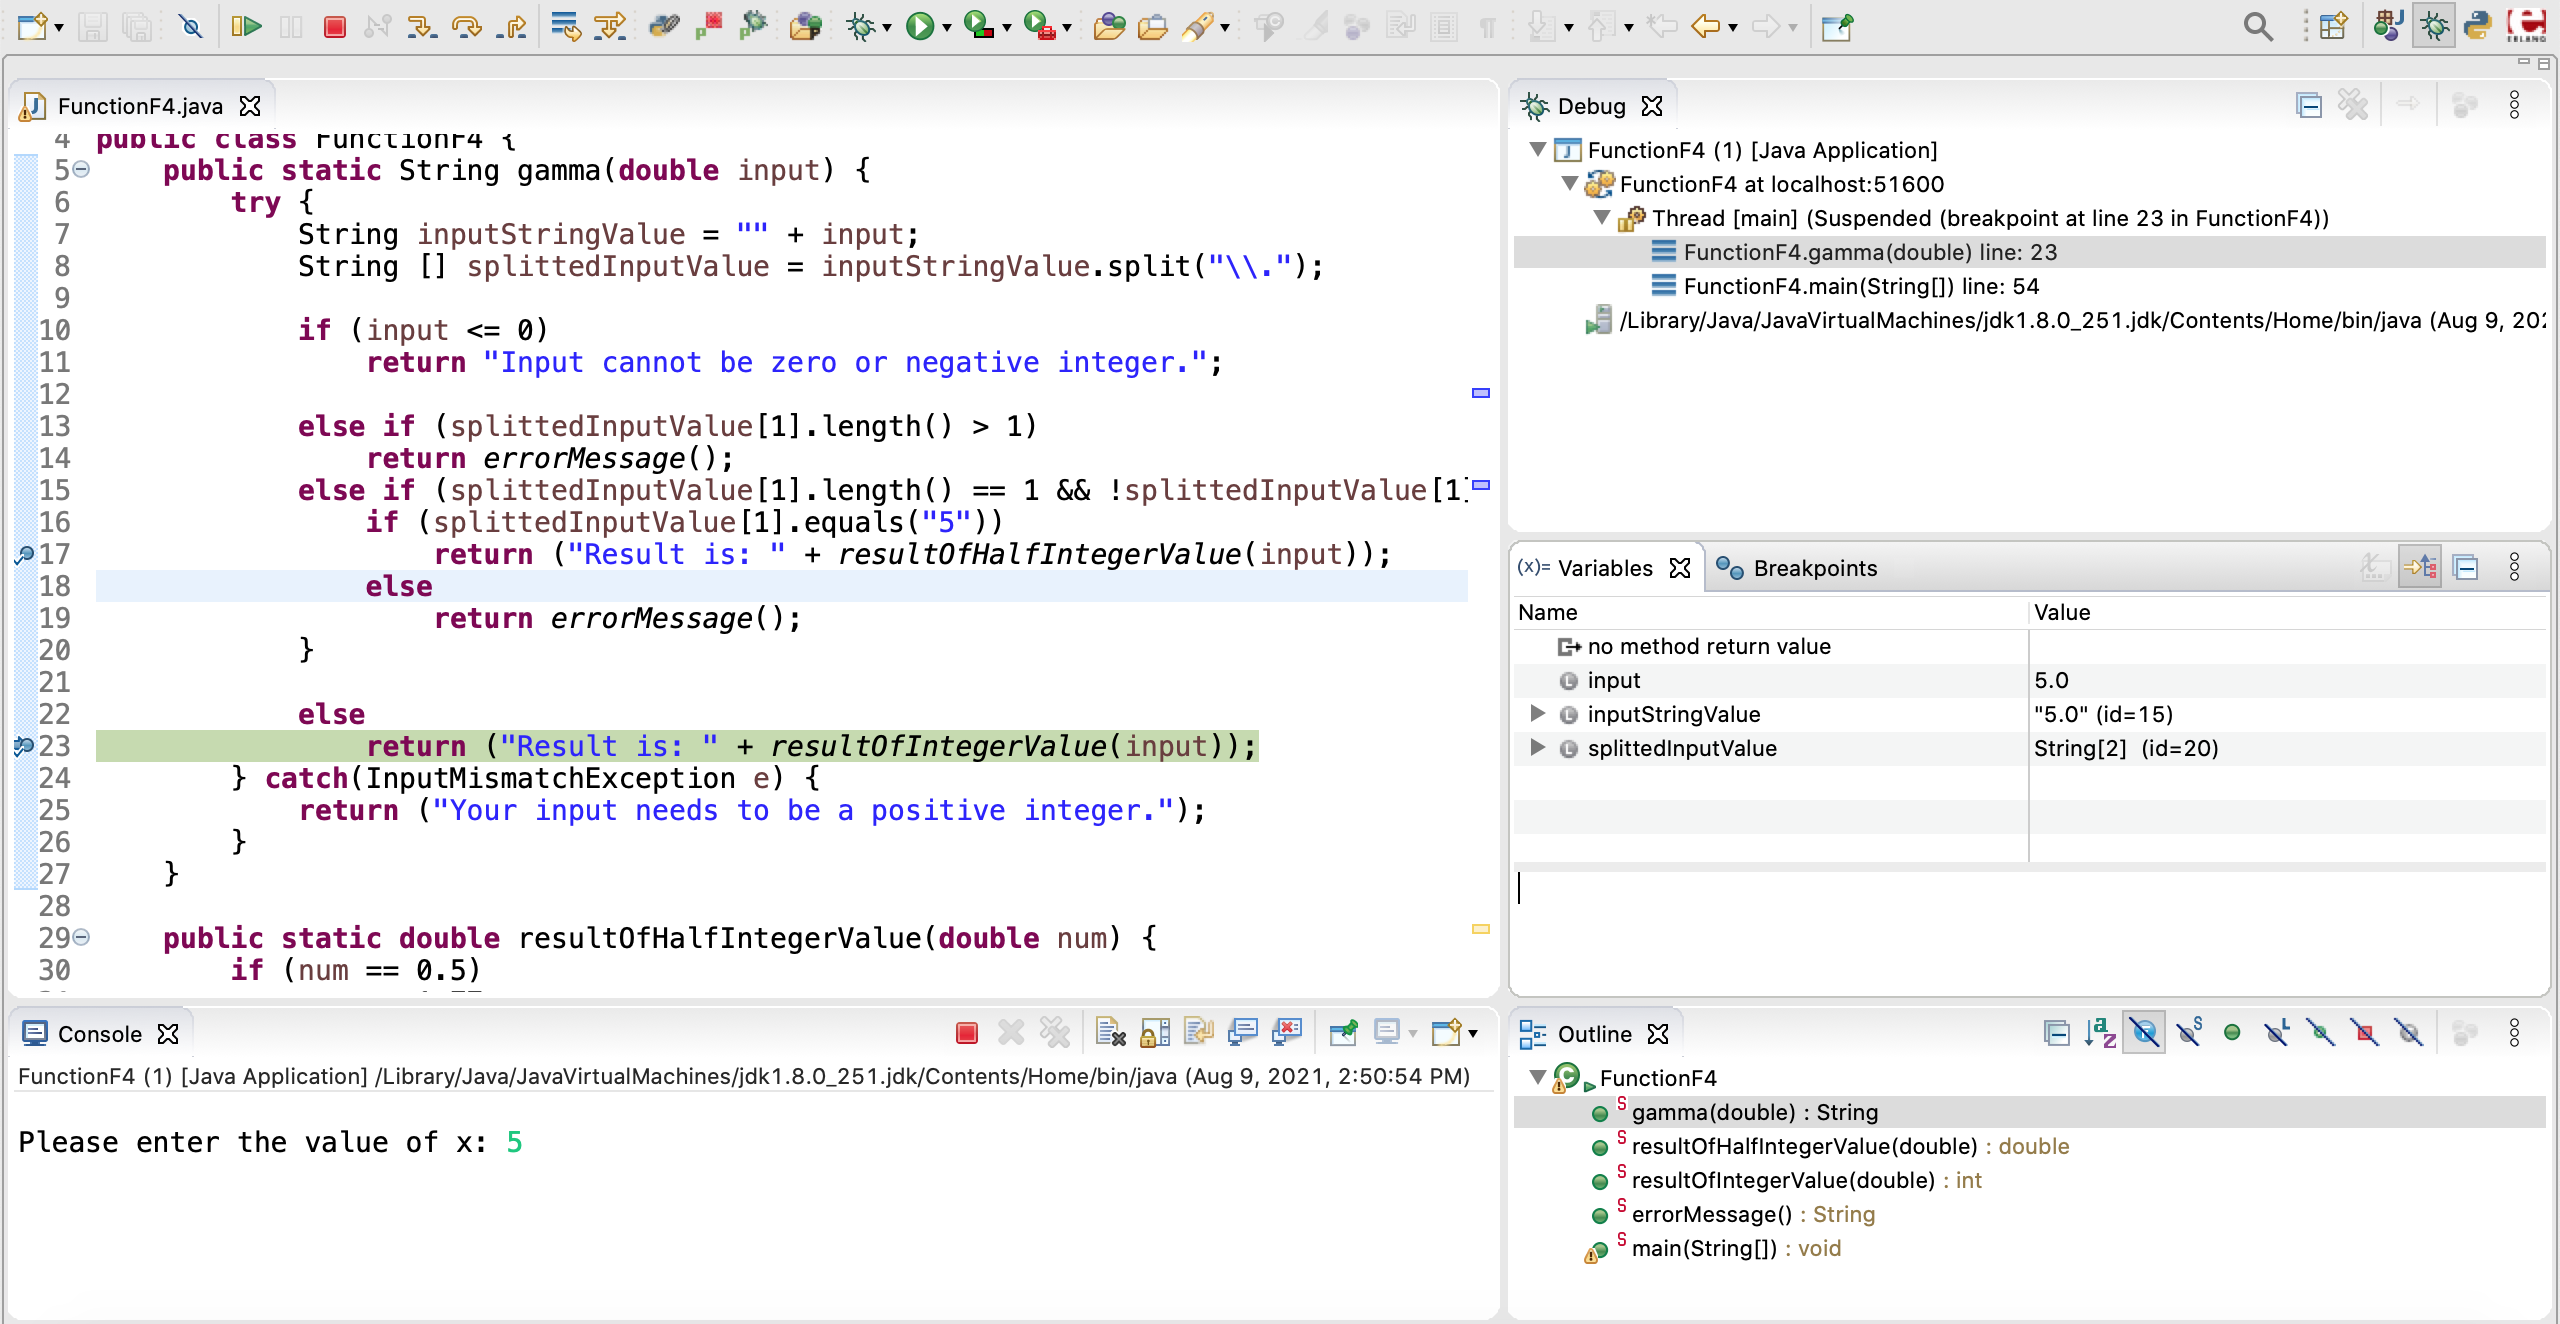
\includegraphics[width=16cm, height=7cm]{debugger.png}
    \subsubsection{Advantages}
    \begin{itemize}
        \item It is free and open source.
        \item It is easy to use – setting breakpoints, executing code line by line, and inspecting the value of variables and expressions.
        \item It also supports other programming languages than Java for investigating and fixing problems with the code.
    \end{itemize}
    \subsubsection{Disadvantages}
    \begin{itemize}
        \item It is usually slower than other debuggers like Visual Studio.
        \item The independent processes cannot be attached to the eclipse debugger to debug.
    \end{itemize}
    
    \newpage
    
    \subsection{Quality Attributes}
    Following are the efforts that has been made in achieving the quality attributes:
    \subsubsection{Correctness}
    \begin{itemize}
        \item ‘Standard’ programming style for the source code has been followed.
        \item Related test cases have been added on the assigned functions.
    \end{itemize}
    
    \subsubsection{Efficient}
    \begin{itemize}
        \item Program takes less time to execute.
        \item Unnecessary variables, methods and the statements have been removed.
    \end{itemize}
    
    \subsubsection{Maintainability}
    \begin{itemize}
        \item Programming style has been made identical throughout the team to remove ambiguity.
        \item Necessary comments have been added where required.
    \end{itemize}
    
    \subsubsection{Robustness}
    \begin{itemize}
        \item Proper error handling has been done for the wrong user inputs.
        \item Use of Try…Catch block for handling java exceptions.
    \end{itemize}
    
    \subsubsection{Usable}
    \begin{itemize}
        \item Simple textual interface has been added for user input and output.
        \item Proper error messages have been given for the wrong inputs.
        \item Proper display of an output has been done for the right inputs.
    \end{itemize}
    
    \newpage
    
    \subsection{CheckStyle}
    I have used the Eclipse plugin - Checkstyle Plug-in 8.44.0 to check the quality of my source code. It is a development tool that helps programmers to write Java code that follows good programming standards. It helps to improve the quality, readability, re-usability of the code and may reduce the development cost.\\
    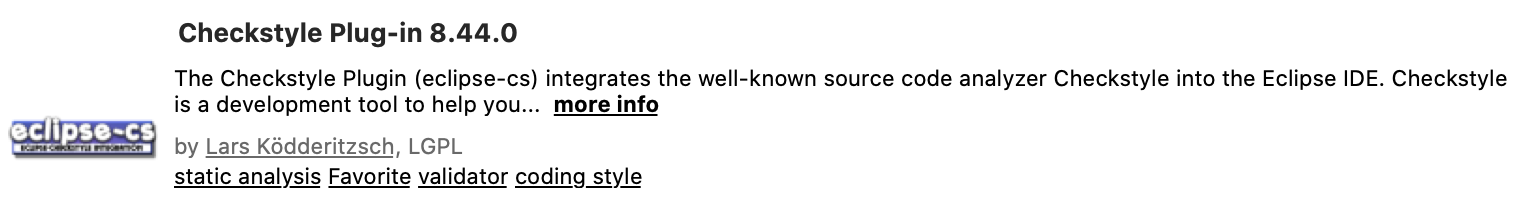
\includegraphics[width=16cm, height=4cm]{check_style.png}
    \subsubsection{Advantages}
    \begin{itemize}
        \item It is portable between IDEs.
        \item It is easier to integrate with external tools as it was designed as a standalone framework.
        \item It has an ability of creating own rules. Eclipse has a large set of styles but checkstyle has more and we can add our own custom rules.
    \end{itemize}
    
    \subsubsection{Disadvantages}
    \begin{itemize}
        \item Checkstyle is limited to a single file static analysis tool.
        \item It is also limited to the presentation of the code and hence does not confirm the correctness or completeness of the code.
    \end{itemize}
    
    \newpage
    
    \section{Problem 5: Source code review of Function F5, ab$^x$}
    \subsection{Introduction}
    The function provided for the source code review purpose was ab$^x$ is a power function. The code was reviewed based on the coding standards that the developer has followed while writing the code. For this, I reviewed coding practices, non-functional requirements and overall structure of the code.
    
    \subsection{Code Review Checklist}
    Following are the checklists of the standard code review guidelines which was used for reviewing the source code:
    \begin{enumerate}
        \item Don’t repeat yourself (Avoid duplication)
        \item Functionality of the code should work properly
        \item Use of meaningful class, method and variables names
        \item Don’t ignore the exception in the code
        \item Avoid creating unnecessary class, methods, variables and objects.
        \item Proper comments have been added
        \item Unnecessary packages should not be imported
        \item Class, function should not be too lengthy
        \item Code must have unit test cases
        \item Proper error message should be displayed
    \end{enumerate}
    
    \subsection{Review Approach}
    Several steps were followed while reviewing the source code.
    \begin{itemize}
        \item First, the code was reviewed well enough to check the naming convention, proper comments in the class and methods, and test cases.
        \item Second, the code was run to check whether the functionality properly works or not.
        \item Third, test cases were run to check whether all the test cases pass or not.
    \end{itemize}
    
    \subsection{Code Review Results}
    \begin{center}
    \begin{tabular}{||c c c||} 
     \hline
     Checklist & Description & Result \\ 
     \hline\hline
     1 & Duplicate Code & PASS \\ 
     \hline
     2 & Functionality of the code & PASS \\
     \hline
     3 & Naming Convention & PASS \\
     \hline
     4 & Exception Handling & PASS \\
     \hline
     5 & No unnecessary class, methods and variables & PASS \\ 
     \hline
     6 & Useful comments & PASS \\
     \hline
     7 & No unnecessary imports & PASS \\
     \hline
     8 & No lengthy code & PASS \\
     \hline
     9 & Must have unit test cases & PASS \\
     \hline
     10 & Proper error message & PASS \\
     \hline
    \end{tabular}
    \end{center}
    
    \subsection{Conclusion}
    From the above, it is noted that the code is well written and all the necessary quality attributes are fulfilled. The only flaw I could found was missing few comments in the function body.
    
    \newpage
    
    \section{Problem 6: Unit Testing - Standard Guidelines}
    \subsection{Description}
    Following are the standard guidelines for implementing unit testing for function F4, $\Gamma(x)$:
    \begin{itemize}
        \item Test case contains the function name used for the unit test case
        \item Test shall cover all cases such as actual and expected value.
        \item For readability, each test case must show proper display message.
        \item Each test cases must be traceable.
        \item Test cases must map all the functional requirements.
    \end{itemize}
    
    \subsection{Implemented Unit Test}
    \begin{itemize}
        \item Junit – a unit testing framework is used.
        \item The sample practice used in the test cases are as follows: \\
            ID: TC1 \\
            Test Case: Description about the test case \\
    \end{itemize}
    
    \newpage
    \section{Problem 7: Testing of Function F7, x$^y$}
    \subsection{Introduction}
    The function provided for the testing purpose is x$^y$ which is a power function. The team member has provided all the required documents to perform the testing of a function.
    \subsection{Test Step}
    \begin{enumerate}
        \item The source code is imported into Eclipse and compiled.
        \item The program is run for different inputs and results were verified.
    \end{enumerate}
    
    \subsection{Test Results}
    \begin{center}
    \begin{tabular}{||c c c||} 
     \hline
     Requirements & Description & Result \\ 
     \hline\hline
     R1 & Valid inputs within the given range & PASS \\ 
     \hline
     R2 & Any base value is raised to the power zero & PASS \\
     \hline
     R3 & Base value zero is raised to any exponent value & PASS \\
     \hline
     R4 & Non-numeric throws exception & PASS \\
     \hline
    \end{tabular}
    \end{center}
    
    \subsection{Conclusion}
    From the above, all the methods of power function are tested and found a positive response. Also, there are no errors found during the testing process. The test cases cover all the requirements as specified in Problem 2. In addition to this, test cases are fast and precise.
\end{document}

